\documentclass{article}
\usepackage{microtype}
\usepackage[utf8]{inputenc} 
\usepackage[a4paper, total={6in, 9.6in}]{geometry}
\usepackage{MnSymbol}
\usepackage{enumerate}
\usepackage{amsmath}
\usepackage{fancyhdr}
\usepackage{xcolor}
\usepackage{tikz}
\usepackage{pgfplots}
\usepackage{marvosym}

\widowpenalties=4 10000 10000 150 0

%% headers
\pagestyle{fancy}
\fancyhf{}
\rhead{Kommunikationssysteme WS19/20}
\lhead{Daniel Schubert, Anton Lydike}
\rfoot{Seite \thepage}

% simple command to display Aufgabe <num>)       ___ / <num>p.
\newcommand\task[1]{\section*{Aufgabe #1)\hfill \underline{\,\,\,\,\,\,}\,\,/1p.}}

% Interpretation (I)
\newcommand\I{I}
% Interpretation und belegung (I, \beta)
\newcommand\Ib{\I, \beta}

%% models
\newcommand\lmodels{\leftmodels} 			% =|
\newcommand\bimodels{\leftmodels\models}	% =||=


%% table for total points
\newcommand\pointsttl[1]{\section*{Gesamtpunkte: \hfill \underline{\,\,\,\,\,\,}\,\,/#1p.}}

%% Funktionen und Prädikate
% Funktionen (arg ist anzahl der stellen)
\newcommand\func[1]{\mathcal{F}^{#1}}
% Prädikate (arg ist anzahl der stellen)
\newcommand\praed[1]{\mathcal{P}^{#1}}

%% Regeln
\newcommand\defrule[2]{\frac{#1}{#2}}

%% Funktionszahl
\newcommand\funcnum[1]{\#_{F}\, #1}

% Für ersetzungen in belegungen wie { x \mapsto d }
\newcommand\repl[2]{\{#1 \mapsto #2\}}

% für alle x .
\newcommand\fall[1]{\forall #1 \, . \,}
\newcommand\ex[1]{\exists #1 \, . \,}

% short biimplication
\newcommand\biimpl{\Leftrightarrow}

% draw a box on the right side of the page
\newcommand\qed{ \hfill $\Box$ }

% red, green, blue text:

\definecolor{greeen}{RGB}{34,139,34}

\newcommand\red[1]{\textcolor{red}{#1}}
\newcommand\green[1]{\textcolor{greeen}{#1}}
\newcommand\blue[1]{\textcolor{blue}{#1}}

% more symbols: https://oeis.org/wiki/List_of_LaTeX_mathematical_symbols

\newcommand\cfgtitle[1]{\title{\vspace{-1.5cm}Übungsblatt #1\\%
\begin{large} Übungsgruppe Metcalfe \end{large}} \lfoot{Übungsblatt #1}\cfoot{Übungsgruppe Metcalfe}}
\author{Daniel Schubert\\Anton Lydike}


%%%%%%%%%%%%%%%%%%%%%%%
%% plotting helpers  %%
%%%%%%%%%%%%%%%%%%%%%%%

%% these draw vertical features
\newcommand\htl[1]{(#1,1) (#1,-1)}  		%% draw line from low to high
\newcommand\lth[1]{(#1,-1) (#1,1)}			%% draw line from high to low

\newcommand\sigtick[2]{\htl{#1} \lth{#2}}	%% draw a htl and then lth line

%% these draw horizontal features
\newcommand\sig[3]{(#2,#1) (#3,#1)}		%% draw a line at height #1 from x=#2 to x=#3
\newcommand\sighi[2]{\sig{1}{#1}{#2}}		%% draw a high signal from #1 to #2
\newcommand\sigmed[2]{\sig{0}{#1}{#2}}		%% draw a null signal from #1 to #2
\newcommand\siglo[2]{\sig{-1}{#1}{#2}}		%% draw a low  signal from #1 to #2


\newcommand\fakeaxis[2]{\addplot [-stealth,black] coordinates {(#1,0) (#2,0)};}



%% units
\newcommand\m{\text{ m}}
\newcommand\s{\text{ s}}
\newcommand\mps{\frac{\text{m}}{\text{s}}}
\newcommand\Gbps{\text{ Gbps}}
\newcommand\bps{\text{ bps}}
\newcommand\bit{\text{ b}}
\newcommand\B{\text{ B}}


\usepackage{multicol,tabularx}
\usepackage{graphicx}
\usepackage{float}
\renewcommand{\arraystretch}{1.5}

\cfgtitle{5}
\date{Mittwoch 27.11.2019}


\renewcommand{\L}{\text{L}}
\newcommand{\R}{\text{R}}
\newcommand\Ssend{\text{S}_{\text{send}}}
\newcommand{\bits}{\text{ b}}

\newcommand\lal[1]{\multicolumn{1}{c|}{#1}}
\newcommand\lale[1]{\multicolumn{1}{c}{#1}}

\renewcommand{\iff}{\Leftrightarrow}

\begin{document}
\maketitle
\thispagestyle{fancy}

\task{1}

\begin{enumerate}[a)]
	\item \begin{tabular}{c|c|c|c|c|c||c|c|c|c|c|c||c|c|c|c|c|c}
	 \multicolumn{6}{c||}{1. Schritt} & \multicolumn{6}{c||}{2. Schritt} & \multicolumn{6}{c}{3. Schritt}  \\ \hline
	  &A&B&C&D&E&   &A&B&C&D&E&   &A&B&C&D&E  \\ \hline
	A &0&1&\infty &\infty &8& A &0&1&3&10&7& A &0&1&3&9&4 \\ \hline
	B & &0&2&\infty &6& B & &0&2&8&3& B & &0&2&5&3  \\ \hline
	C & & &0&\infty &1 & C & & &0&3&1& C & & &0&3&1 \\ \hline
	D & & & &0&2& D & & & &0&2& D & & & &0&2   \\ \hline
	E & & & & &0& E & & & & &0& E & & & & &0  \\ 
	
	\end{tabular}
	
	
	\item Beste ist $D_B(C)=4$, aber beste richtige ist $D_B(C)=7$
	
	\item 
	
	\begin{tabular}{l|l|l|l|l|l}
	\lal{Iteration} & \lal{N'}&\lal{D(B), p(B)}  & \lal{D(C), p(C)}  & \lal{D(D), p(D)}  & \lale{D(E), p(E)}  \\ \hline
	0         &A        &1, A          &\infty       &\infty       &8, A          \\
	1         &A, B      &1, A          & 3, B         &10, E         &7, B          \\
	2         &A, B, C    & 1 ,A         & 3, B         &10, E         &7, B          \\
	3         &A, B, C, E  & 1, A         & 3, B         &9, E          &4, C          \\
	4         &A, B, C, E, D& 1, A         & 3, B         &6, E          &4, C          \\
	
	
	\end{tabular}
\end{enumerate}

\task{2}


\begin{enumerate}[a)]
\item 
	\begin{enumerate}[1)]
		\item $B \overset{2}{\to} A \overset{3}{\to} D$
		\item $D \overset{3}{\to} A \overset{2}{\to} B  \overset{1}{\to} E$
		\item $C \overset{2}{\to} A \overset{3}{\to} D$
		\item $B \overset{2}{\to} A \overset{3}{\to} D$
	\end{enumerate}

	\begin{figure}[H]
		\centering
		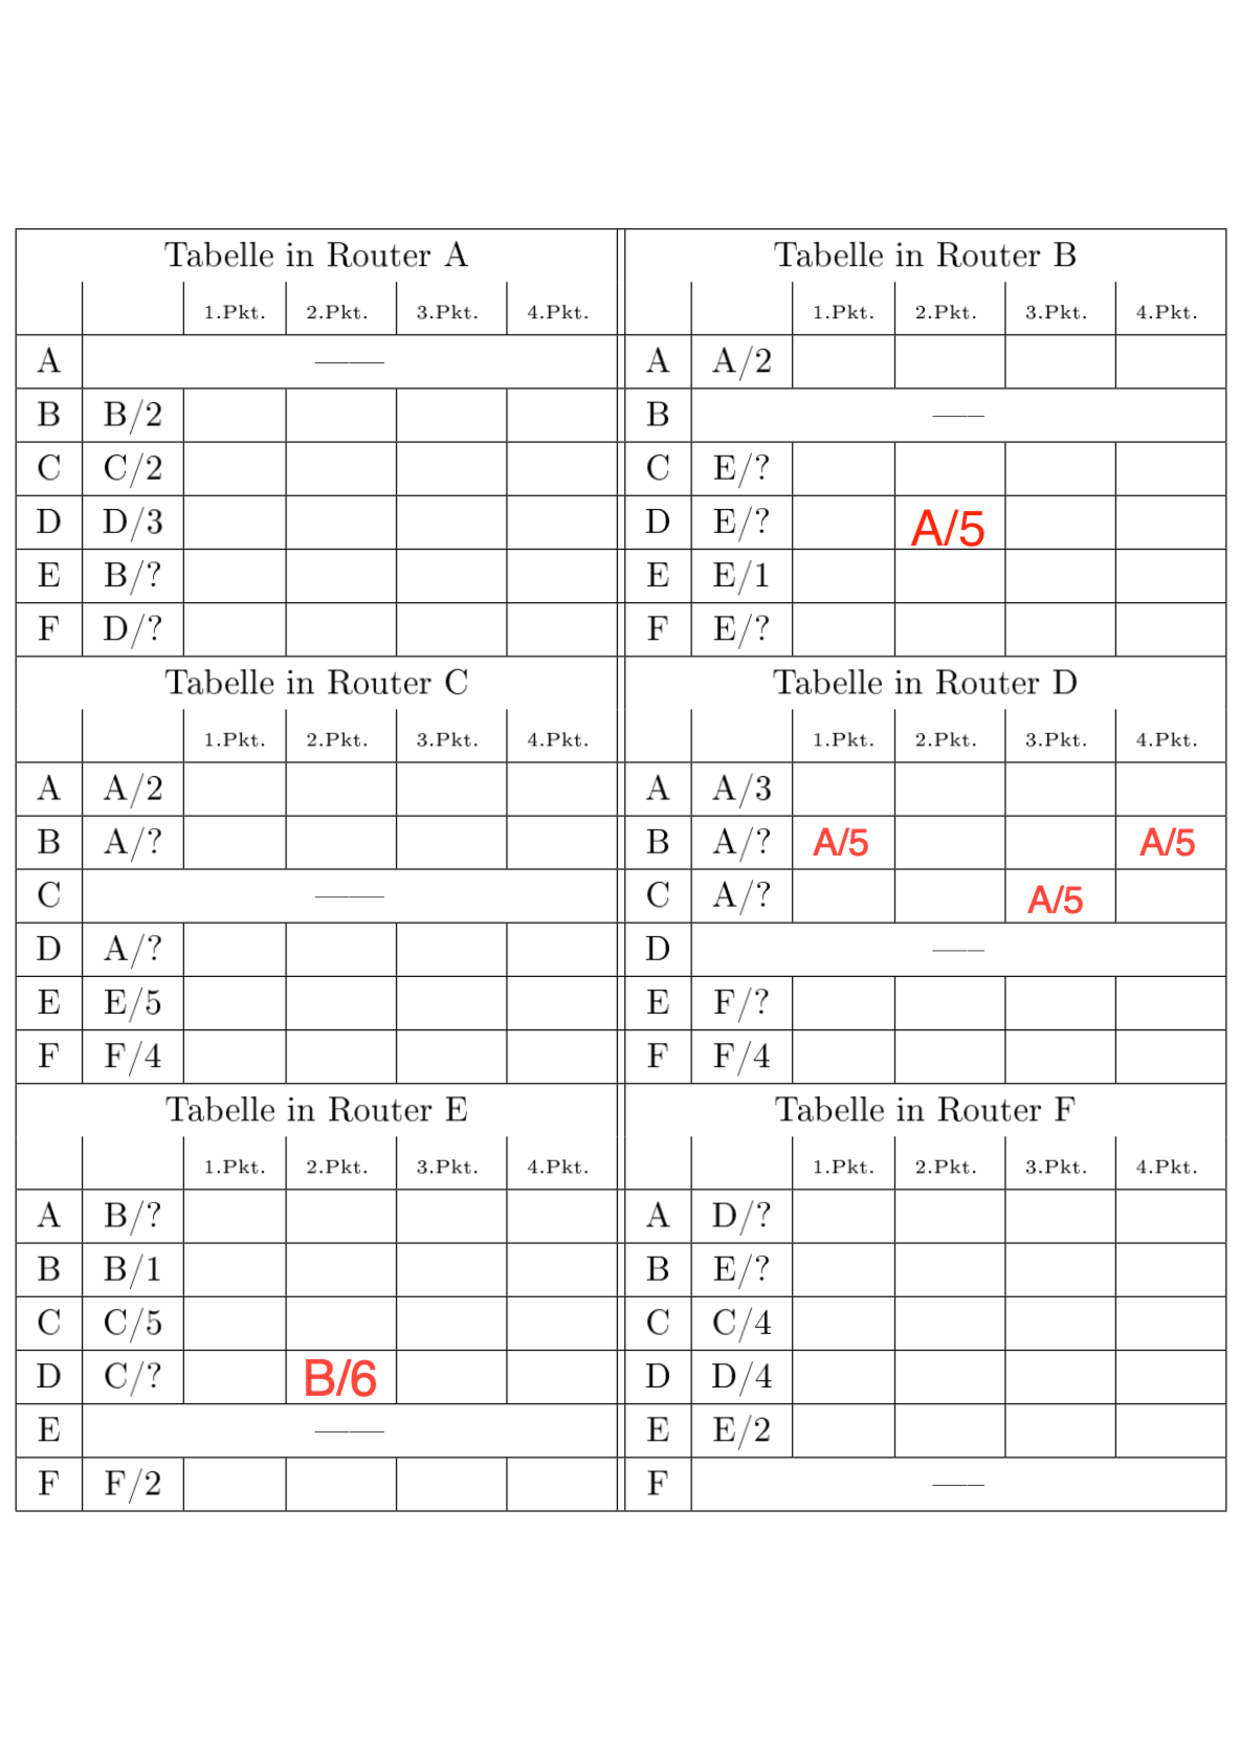
\includegraphics[trim = 0cm 4cm 0cm 4cm,width=13cm]{table.pdf}
	\end{figure}

\item \begin{itemize}


		\item Während der Lernperiode ist das Routing nicht optimal.
		\item Da Ausfälle/Überlastungen nicht mitgeteilt werden, müssen tabellen periodisch alle informationen vergessen und neu initialistert werden.	
	
	\end{itemize}

\end{enumerate}

\task{3}

\begin{enumerate}[a)]

\item Bei der \textit{verbindungsorientierten Kommunikation} ist eine Wegsuche Notwendig und die Sendereihenfolge wird strikt eingehalten. Bei der \textit{verbindungslosen Kommunikation} wird keine Wegsuche betrieben, stattdessen werden die Pakete einfach einzeln auf die Reise geschickt und können unterschiedliche Pfade beschreiten. Hierbei verlässt man sich auf die Entscheidungen der Router auf dem Weg.
\item 
	\begin{itemize}
		\item Richtig
		\item Richtig
		\item Falsch, da die Packetvermittlung ein Oberbegriff für verschiedene Strategien ist. Es existieren Packetvermittlungen, für welche die Aussage stimmt, und andere, für die das nicht gilt.
		\item Falsch
	\end{itemize}

\item \textit{Broadcast} ist eine Nachricht an alle erreichbaren Hosts, während ein \textit{Multicast} nur an ein subset der erreichbaren Hosts adressiert ist.
\item \textit{HELLO-Pakete} werden verwendet, um festzustellen, ob ein Netzwerkpartner noch am Leben ist. Außerdem werden sie von neuen Netzwerkteilnehmern emitiert, wenn sie einem Netzwerk beitreten. \textit{Link-State-Advertisement} wird verwendet, um deine direkten Nachbarn (zusammen mit den Kosten der Verbindung) an die große, weite Welt zu broadcasten.
\item
	\begin{tabular}{r c c}
					& \textit{Link-State} & \textit{Backwards Learning} \\
		StatischesRouting: & \bigcirc     & $\bigotimes$ \\
		AdaptivesRouting:  & $\bigotimes$ & \bigcirc \\
		VerteiltesRouting: & $\bigotimes$ & $\bigotimes$ \\
		IsoliertesRouting: & \bigcirc     & $\bigotimes$ \\
	\end{tabular}

\end{enumerate}

\pointsttl{3}


\end{document}
